%% Fig. 2 -- system architecture. Rendered to architecture.png by ../build-figures.sh
\documentclass[border=4pt]{standalone}
\usepackage{times}
\usepackage{tikz}
\usetikzlibrary{arrows.meta,positioning,shapes.geometric}
\newcommand{\pkg}[1]{\texttt{#1}}

\begin{document}
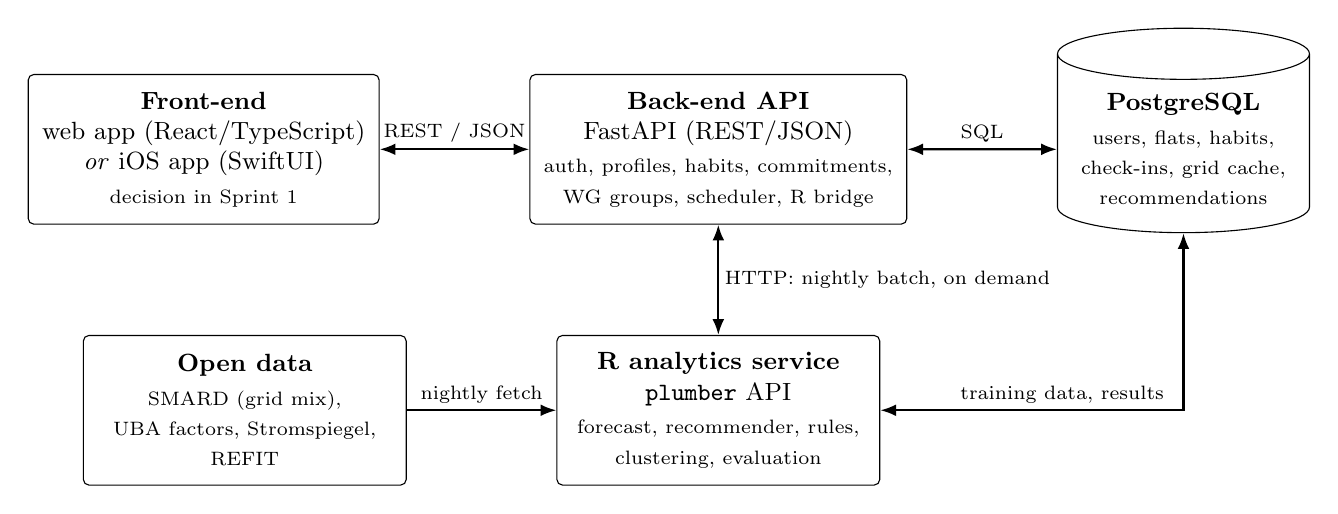
\begin{tikzpicture}[
  node distance=11mm and 19mm,
  box/.style={draw, rounded corners=2pt, align=center, minimum height=1.9cm,
              minimum width=4.1cm, inner sep=5pt, font=\small},
  data/.style={draw, cylinder, shape border rotate=90, aspect=0.22, align=center,
               minimum height=1.9cm, minimum width=3.2cm, inner sep=5pt, font=\small},
  arr/.style={-{Latex[length=2mm]}, thick},
  darr/.style={{Latex[length=2mm]}-{Latex[length=2mm]}, thick},
  lbl/.style={font=\scriptsize, inner sep=2pt}]
\node[box] (fe) {\textbf{Front-end}\\ web app (React/TypeScript)\\ \emph{or} iOS app (SwiftUI)\\[1pt] \scriptsize decision in Sprint 1};
\node[box, right=of fe] (be) {\textbf{Back-end API}\\ FastAPI (REST/JSON)\\[1pt] \scriptsize auth, profiles, habits, commitments,\\ \scriptsize WG groups, scheduler, R bridge};
\node[data, right=of be] (db) {\textbf{PostgreSQL}\\[1pt] \scriptsize users, flats, habits,\\ \scriptsize check-ins, grid cache,\\ \scriptsize recommendations};
\node[box, below=14mm of be] (r) {\textbf{R analytics service}\\ \pkg{plumber} API\\[1pt] \scriptsize forecast, recommender, rules,\\ \scriptsize clustering, evaluation};
\node[box, left=of r] (od) {\textbf{Open data}\\[1pt] \scriptsize SMARD (grid mix),\\ \scriptsize UBA factors, Stromspiegel,\\ \scriptsize REFIT};
\draw[darr] (fe) -- node[lbl, above] {REST / JSON} (be);
\draw[darr] (be) -- node[lbl, above] {SQL} (db);
\draw[darr] (be) -- node[lbl, right] {HTTP: nightly batch, on demand} (r);
\draw[arr] (od) -- node[lbl, above] {nightly fetch} (r);
\draw[darr] (r.east) -| node[lbl, pos=0.3, above] {training data, results} (db.south);
\end{tikzpicture}
\end{document}
